\subsection{Richard's Frequenztransformation}

Das LC-Filter von der Abbildung  \ref{fig:Topologie_Prototyp.png} wird nun mit
der  Richards-Frequenztransformation   in   Stichleitungen   umgewandelt.  Die
Grenzfrequenz $f_c$ ist dabei \SI{0.8}{\giga\hertz} und die Bezugsfrequenz $f$
ist \SI{2}{\giga\hertz}.

\begin{equation}
    \Omega = \tan\frac{\pi}{2}\frac{f_c}{f}
\end{equation}

Die entnormierten Leitungsimpedanzen (mit einer eingangs- und Ausgangsimpedanz
von  \SI{50}{\ohm}) werden  von  den  g-Parameter  nun  wie  folgt  berechnet.

\begin{align*}
    R_0 &= 50 g_0               & L_4 &= \frac{50g_4}{\Omega} \\ 
    C_1 &= \frac{g_1}{50\Omega} & C_5 &= \frac{g_5}{50\Omega} \\ 
    L_2 &= \frac{50g_2}{\Omega} & R_6 &= 50 g_6               \\ 
    C_3 &= \frac{g_3}{50\Omega} &     &                       \\
\end{align*}

Die  Abbildung  \ref{fig:stripline-richards}  zeigt,  wie die Kapazit\"aten in
TLOCs   und   die   Inuktivit\"aten   in   TLSCs   umgewandelt  worden   sind.

\begin{figure}[h!]
    \centering
    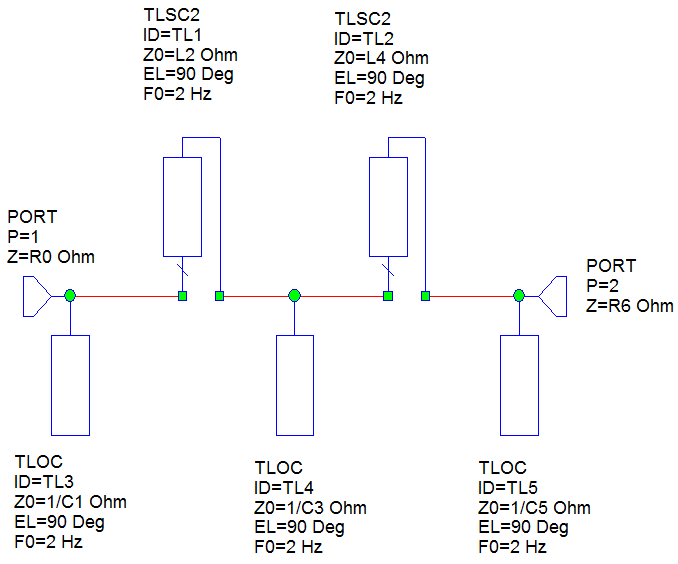
\includegraphics[width=\imagewidth]{images/stripline-richards}
    \caption{Resultierende Umwandlung des LC-Filters in Stichleitungen mithilfe der Richards-Transformation.}
    \label{fig:stripline-richards}
\end{figure}

Der Amplitudengang und Reflexion ist in der Abbildung \ref{fig:graph-richards}
ersichtlich.  Vergleicht  man  das Verhalten des Filters mit dem Verhalten des
LC-Filters  in  Abbildung  \ref{fig:graph-LC},  so   wird   man  eine  leichte
Verzerrung  feststellen,  welches um die Bezugsfrequenz vernachl\"assigbar ist
aber  weiter  davon  entfernt  (zum  Beispiel  bei  \SI{3}{\giga\hertz})  viel
signifikanter wird.

\begin{figure}[h!]
    \centering
    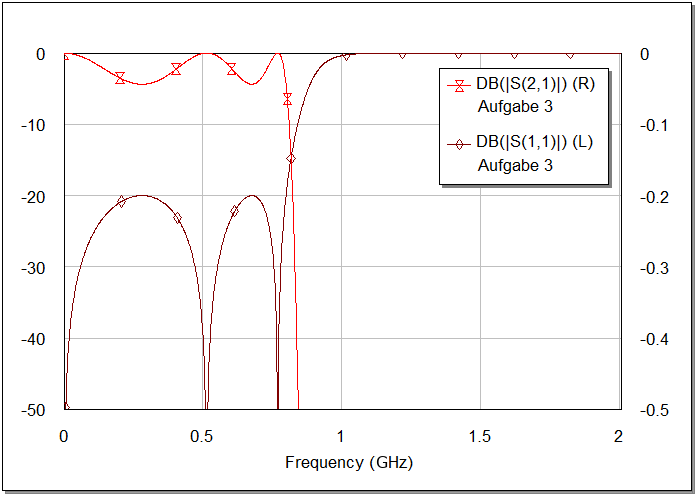
\includegraphics[width=\imagewidth]{images/graph-richards}
    \caption{Filterverhalten des Filters nach der Richards-Frequenztransformation (Amplitudengang S21 und Reflexion S11)}
    \label{fig:graph-richards}
\end{figure}

